% Diese Datei ist Teil des Buchs "Schreibe Dein Programm!"
% Das Buch ist lizensiert unter der Creative-Commons-Lizenz
% "Namensnennung - Weitergabe unter gleichen Bedingungen 4.0 International (CC BY-SA 4.0)"
% https://creativecommons.org/licenses/by-sa/4.0/deed.de

% FIXME: Referenz auf RC_1 / logische Kalküle
% FIXME: "Reduktionskalkül" erklären
\chapter{Exkurs: Der $\lambda$-Kalkül}
\label{chap:lambda}

\newcommand{\lrm}{\mathrm}

\index{Lambda-Kalkül@$\lambda$-Kalkül}

Bisher ging es in diesem Buch immer um die \emph{Konstruktion} von
Programmen.  In dieses Kapitel geht es hingegen um die
\textit{Bedeutung} von Programmen.  Wir haben zwar erläutert, wie die
Auswertung eines Programms funktioniert, aber bisher nur
umgangssprachlich.  Dabei haben wir einige subtile Aspekte der
Auswertung gar nicht oder nur unpräzise erläutert.  Das wollen wir in
diesem Kapitel korrigieren und zwar mit Mathematik~-- wie immer, wenn
es wirklich präzise sein muss.

Dazu benutzen wir den sogenannten \textit{$\lambda$-Kalkül},
ausgeschrieben: \textit{Lambda-Kalkül}, der formal fasst, was der
Stepper in DrRacket visualisiert.  Das "<Lambda"> im Namen des Kalküls
ist die Vorlage für das \lstinline{lambda} in unseren Lehrsprachen.
Der $\lambda$-Kalkül bricht die Elemente der Programmierung auf nur
das absolut notwendige herunter, das macht ihn glücklicherweise
ziemlich einfach.  Gleichzeitig kann er alles abbilden, was wir für
die Programmierung so brauchen.

\section{Die Sprache des $\lambda$-Kalküls}
\label{sec:sprache}

Ein mathematischer \textit{Kalkül}\index{Kalkül} dient im allgemeinen
dazu, Aussagen hinzuschreiben und wahre Aussagen herzuleiten.  Wir
wollen Aussagen über Programme machen und was sie bedeuten.  Damit es
losgeht, benötigen zunächst eine \textit{Sprache} für den Kalkül, und
den definieren wir mit Hilfe einer Grammatik.  (Du erinnerst Dich
vielleicht, das ist eine Notation für induktive Definitionen, die wir
in Abschnitt~\ref{sec:grammatik} auf Seite~\pageref{sec:grammatik}
eingeführt haben.)

Die folgenden Definition definiert als Grundlage für die Sprache des
$\lambda$-Kalküls die Sprache der $\lambda$-Terme.  Wie wir sehen
werden, entsprichen die Terme den Ausdrücken in unseren Programmen. 

In der Definition taucht der Begriff \textit{abzählbare
  Menge}\index{abzählbare Menge} auf.  Das Adjektiv "<abzählbar"> an
einer Menge bedeutet, dass die Menge unendlich groß ist und dass die
Menge durchnummeriert oder "<abgezählt"> werden kann.  Hier geht es um
die abzählbare Menge der Variablen, welche den Variablen in Programmen
entsprechen.  Die könnten wir auch durchnummerieren, indem wir den
Buchstaben Nummern geben.

\begin{definition}[Sprache des $\lambda$-Kalküls
  $\mathcal{L}_{\lambda}$]
  
  Sei $V$ eine abzählbare Menge von Variablen. 
  Die Sprache des $\lambda$"=Kalküls, die Menge der
  \textit{$\lambda$-Terme\index{Lambda-Term@$\lambda$-Term}},
  $\mathcal{L}_{\lambda}$\index{L@$\mathcal{L}_{\lambda}$}, ist
  durch folgende Grammatik definiert:
  \begin{grammar}
    \meta{$\mathcal{L}_{\lambda}$} \: \meta{$V$}
    \> \| ($\mathcal{L}_{\lambda}$ $\mathcal{L}_{\lambda}$)
    \> \| ($\lambda$\meta{$V$}.$\mathcal{L}_{\lambda}$)
  \end{grammar}
%
  Ein $\lambda$-Term der Form $(e_0~e_1)$ heißt
  \textit{Applikation\index{Applikation}}. Ein Term der Form
  $(\lambda v.e)$ heißt \textit{Abstraktion\index{Abstraktion}}, wobei
  $v$ \textit{Parameter\index{Parameter}} der Abstraktion heißt und
  $e$ \textit{Rumpf\index{Rumpf}}.
\end{definition}
%
Hier sind ein paar Beispiele für $\lambda$-Terme:
%
\begin{displaymath}
  \begin{array}{c}
    (\lrm f~\lrm x)
    (\lambda \lrm x.\lrm x)\\
    (\lambda \lrm x.(\lambda \lrm y.(\lrm x~\lrm y))\\
    (\lambda \lrm x.(\lrm f~\lrm x))\\
    (\lambda \lrm x.(\lrm f~(\lambda \lrm x~\lrm x))
  \end{array}
\end{displaymath}
% 
In diesen konkreten Beispielen haben wir als Variablen $\lrm x$, $\lrm y$ und
$\lrm f$ verwendet.  Manchmal sprechen wir aber auch über
$\lambda$-Terme einer bestimmten Form im Allgemeinen, zum Beispiel
steht oben in der Definition "<$\lambda$-Term der Form
$(e_0~e_1)$">. Damit sind \emph{alle} $\lambda$-Terme gemeint, die aus der
zweiten Regel der Grammatik stammen, also $e_0$ und $e_1$ beliebige
$\lambda$-Terme sein können.  Hier sind einige Beispiele für
$\lambda$-Terme dieser Form:
%
\begin{displaymath}
  \begin{array}{c}
    (\lrm f~\lrm x)
    (\lrm f~(\lambda \lrm x.\lrm x))
    ((\lambda \lrm x.\lrm x)~(\lambda \lrm x.\lrm x))
  \end{array}
\end{displaymath}
%
In der Definition sind außerdem Terme der "<Form $(\lambda v.e)$>
erwähnt, das könnte zum Beispiel sein:
%
\begin{displaymath}
  \begin{array}{c}
    (\lambda \lrm x.\lrm x)
    (\lambda \lrm y.\lrm x)
    (\lambda \lrm x.\lrm x~\lrm x)
    (\lambda \lrm x.(\lrm f~\lrm x)~\lrm y)
    (\lambda \lrm y.\lrm x)
  \end{array}
\end{displaymath}
%
Du sieht, der Buchstabe $v$ in der "<Form> steht für eine Variable,
also für $\lrm x$, $\lrm y$ oder $\lrm f$.  Wenn Du genau hinschaust,
siehst Du, dass beide sich typografisch unterscheiden: Die
"<normalen"> Variablen $\lrm x$, $\lrm y$, $\lrm f$ sehen aus wie
reguläre Buchstaben, während $v$ in sogenannten Italics gesetzt ist.
Das $v$ ist also eine Variable, die für eine andere Variable steht~--
eine sogenannte \textit{Metavariable}.\index{Metavariable}

In diesem Kapitel steht die Variable $e$ immer für einen
$\lambda$-Term, $u$, $v$ und $w$ sind immer Metavariablen.

Anders als in den Lehrsprachen werden Klammern bei $\lambda$-Termen
oft weggelassen.  Statt des vollständig geklammerten Terms

\begin{displaymath}
  (\lambda \lrm f.(\lambda \lrm x.(\lrm f~\lrm x)))
\end{displaymath}
%
werden wir das hier schreiben: 
%
\begin{displaymath}
  \lambda \lrm f.\lambda \lrm x.\lrm f~\lrm x
\end{displaymath}
%
Prinzipiell lässt sich dieser Term unterschiedlich
klammern: $(\lambda \lrm f.((\lambda \lrm x.\lrm f)~\lrm x))$, $(\lambda
f.(\lambda \lrm x.(\lrm f~\lrm x)))$ oder $((\lambda \lrm f.\lambda
\lrm x.\lrm f)~\lrm x)$.  Wir verwenden aber die gängige Konvention,
dass der Rumpf einer Abstraktion sich so weit wie möglich nach
rechts erstreckt.   Damit steht der ungeklammerte Term eindeutig für
den vollständig geklammerten Term, der darüber steht.

Die Terme der Form $\lambda v.e$ sind auf einen Parameter
beschränkt.  Es gibt aber zwei weitere Abkürzungen
in der Notation von $\lambda$-Termen:
%
\begin{itemize}
\item $\lambda x_1 \ldots x_n.e$ steht für $\lambda x_1.(\lambda
  x_2.(\ldots\lambda x_n.e)\ldots)$.
\item $e_0 \ldots e_n$ steht für $(\ldots(e_0~e_1)~e_2) \ldots e_n)$.
\end{itemize}
%
Dementsprechend ist $\lambda \lrm{fxy}.\lrm f~\lrm x~\lrm y$ eine andere Schreibweise für
den Term \[(\lambda \lrm f.(\lambda \lrm x.(\lambda \lrm y.((\lrm f~\lrm x)~\lrm y))))\ .\]

\section{$\lambda$-Intuition}

Es ist kein Zufall, dass die Lehrsprachen genau die gleichen Begriffe verwenden
wie der $\lambda$-Kalkül.  Ein Lambda-Ausdruck mit einem
Parameter entspricht einer Abstraktion im $\lambda$-Kalkül,
und die Applikationen in den Lehrsprachen entsprechen den Applikationen im
$\lambda$-Kalkül.  Die Lehrsprachen wurde bewusst auf dem
$\lambda$-Kalkül aufgebaut.

Die Intuition für die Bedeutung der $\lambda$-Terme ist ähnlich wie in
den Lehrsprachen: Eine Abstraktion steht für eine mathematische Funktion,
speziell für eine solche Funktion, die sich durch ein Computerprogramm
berechnen lässt.\footnote{Die Wahl des Buchstabens $\lambda$ für die
  Notation von Abstraktionen war eher ein Unfall: Zur Zeit der
  Entstehung des Kalküls war der Ausdruck $2\hat{x}+1$ eine historische Notation für eine
  Funktion $f$ mit $f(x)\deq{}2x+1$.  \textsc{Alonzo Church},
  der Erfinder des $\lambda$-Kalküls, hatte ursprünglich
  die Notation $\hat{x}.2x+1$ in der ersten Publikation über den
  Kalkül vorgesehen.  Der Schriftsetzer konnte allerdings aus
  technischen Gründen
  das Hütchen nicht über dem $x$ positionieren und setzte es deshalb
  davor, womit aus dem Ausdruck $\hat{~}\thinspace{}x.2x+1$ wurde.  Ein weiterer
  Setzer machte aus dem einsamen Hütchen ein $\lambda$ und der
  $\lambda$-Kalkül war geboren.}  Eine Applikation steht gerade für
die Applikation einer Funktion, und eine Variable bezieht sich auf den
Parameter einer umschließenden Abstraktion und steht für den Operanden
der Applikation.  

Wichtig ist aber: Das ist an diesem Punkt nur eine Intuition.  Wir
haben bisher nur die Sprache des $\lambda$-Kalküls definiert, nicht
aber, was die $\lambda$-Terme bedeuten oder wie sie sich verhalten.

Bemerkenswert am $\lambda$-Kalkül ist, dass es dort \emph{nur}
Funktionen gibt, noch nicht einmal Zahlen, boolesche Werte oder
zusammengesetzte Daten.  Darum erscheint die Sprache des Kalküls auf den
ersten Blick noch spartanisch und unintuitiv: So unmittelbar lässt sich
noch nicht einmal eine Funktion hinschreiben, die zwei Zahlen addiert~--
schließlich gibt es keine Zahlen.  Wie sich jedoch weiter unten in
Abschnitt~\ref{sec:lambdaprog} herausstellen wird, lassen sich all diese
Dinge durch Funktionen nachbilden.

Noch etwas: Es gibt nur Funktionen, und die haben auch nur jeweils
einen Parameter.  Dies ist aber keine wirkliche Einschränkung:
Funktionen mit mehreren Parametern können wir
schönfinkeln\index{schönfinkeln}, um aus ihnen mehrstufige
Funktionen mit jeweils einem Parameter zu machen, wie schon in
Abschnitt~\ref{sec:currying} auf Seite~\pageref{sec:currying}.

\section{Wie funktionieren Variablen?}

Im $\lambda$-Kalkül dreht sich (fast) alles um Variablen.  Die
funktionieren nach dem gleichen Prinzip wie bei den Lehrsprachen, der
lexikalischen Bindung.  Die lexikalische Bindung haben wir in
Abschnitt~\ref{sec:lexikalische-bindung} auf
Seite~\pageref{sec:lexikalische-bindung} behandelt.  Kurz zur
Erinnerung:  Das
Vorkommen einer Variable $v$ als $\lambda$-Term gehört immer zur
innersten umschließenden Abstraktion $\lambda v.e$, deren Parameter
ebenfalls $v$ ist.  Bei $\lambda \lrm x.\lrm y~(\lambda \lrm y.\lrm y))$ 
ist also das erste $y$ das freie, während das zweite $y$ durch
die zweite Abstraktion gebunden wird.

Dieses Prinzip erklärt aber nicht die Mechanik, wie für Variablen
Werte eingesetzt werden.  Um die präzise zu definieren, brauchen wir
zwei Hilfsfunktionen für den Umgang mit Variablen.
%
\begin{definition}[Freie und gebundene Variablen]
  Die Funktionen $\free$ und $\bound$ liefern für einen
  $\lambda$-Terms die Mengen seiner \emph{freien} beziehungsweise seiner
  \emph{gebundenen} Variablen.  \index{Variable!frei}\index{freie
    Variable}\index{Variable!gebunden}\index{gebundene Variable}%
  \index{free@$\free$}\index{bound@$\bound$}
  %
  \begin{align*}
    \free(e) & \deq
    \begin{cases}
      \{ v \}  & \text{falls } e  = v\\
      \free(e_0) \cup \free(e_1) & \text{falls } e = e_0~e_1\\
      \free(e_0) \setminus \{v\} & \text{falls } e = \lambda v.e_0
    \end{cases}\\
    \bound(e) & \deq
    \begin{cases}
      \varnothing & \text{falls } e = v\\
      \bound(e_0) \cup \bound(e_1) & \text{falls } e = e_0~e_1\\
      \bound(e_0) \cup \{v\} & \text{falls } e = \lambda v.e_0
    \end{cases}
  \end{align*}
  %
  Ein
  $\lambda$-Term $e$ heißt \emph{abgeschlossen\index{abgeschlossen}} beziehungsweise 
  \textit{Kombinator\index{Kombinator}}, falls $\free(e)=\varnothing$.
\end{definition}
%
Einige Beispiele:
%
\begin{eqnarray*}
  \free(\lambda \lrm x.\lrm y) &=& \{\lrm y\}\\
  \bound(\lambda \lrm x.\lrm y) &=& \{\lrm x\}\\
  \free(\lambda \lrm y.\lrm y) &=& \varnothing\\
  \bound(\lambda \lrm y.\lrm y) &=& \{\lrm y\}\\
  \free(\lambda \lrm x.\lambda \lrm y.\lambda \lrm x.\lrm x~(\lambda \lrm z.\lrm a~\lrm y)) &=& \{ \lrm a\}\\
  \bound(\lambda \lrm x.\lambda \lrm y.\lambda \lrm x.\lrm x~(\lambda z.\lrm a~\lrm y)) &=& \{ \lrm x,\lrm y,\lrm z\}
\end{eqnarray*}
%
Die Intuition ist folgende: Eine Abstraktion in einem $\lambda$-Term
\emph{bindet} eine Variable innerhalb seines Rumpfes.  Eine freie
Variable hingegen ist eine, die nicht durch eine Abstraktion gebunden
ist.  Darum subtrahiert $\free$ bei einer Abstraktion die gebundene
Variable.  Dahingegen sammelt $\bound$ alle Variablen aus
Abstraktionen auf.  Wenn man $\free$ und $\bound$ eines Terms als
$\free(e)\cup\bound(e)$ zusammennimmt, bekommt man alle Variablen
eines $\lambda$-Terms enthält.

In einem Term kann die gleiche Variable sowohl frei als auch gebunden
vorkommen:
%
\begin{eqnarray*}
  \free(\lambda \lrm x.\lrm y~(\lambda \lrm y.\lrm y)) &=& \{ \lrm y\} \\
  \bound(\lambda \lrm x.\lrm y~(\lambda \lrm y.\lrm y)) &=& \{ \lrm x,
                                                            \lrm y\}
\end{eqnarray*}
%
Das $\lrm y$ taucht einmal innerhalb und einmal außerhalb einer bindenden
Abstraktion auftaucht. Das Frei- und Gebundensein bezieht sich also
immer auf bestimmte Vorkommen\index{Vorkommen} einer Variablen in
einem $\lambda$-Term.

Der $\lambda$-Kalkül ist darauf
angewiesen, Variablen durch andere zu ersetzen, ohne dabei die
Zugehörigkeit von Variablenvorkommen und den dazu passenden
Abstraktionen zu verändern.  Der Mechanismus dafür heißt auch hier
\textit{Substitution}:
%
\begin{definition}[Substitution]\index{Substitution}
  Für $e,f\in \mathcal{L}_{\lambda}$ ist $e[v\mapsto f]$~-- in $e$ wird $v$ durch $f$
  \textit{substituiert}~-- induktiv definiert:\index{*@$\mapsto$}

  \begin{displaymath}
    e[v\mapsto f] \deq
    \begin{cases}
      f & \text{falls } e = v\\
      x & \text{falls } e = x \text{ und } x \neq v\\
      \lambda v.e_0 & \text{falls } e = \lambda v.e_0\\
      \lambda u.(e_0[v\mapsto f]) & \text{falls } e = \lambda u.e_0 \text{
        und } u\neq v, u\not\in\free(f)\\
      \lambda u'.(e_0[u\mapsto u'][v\mapsto f]) & \text{falls }
      e = \lambda u.e_0 \\ & \text{und }
      u \neq v,u\in\free(f), u'\not\in\free(e_0)\cup\free(f)\\
      (e_0[v\mapsto f])~(e_1[v\mapsto f]) &
      \text{falls } e = e_0~e_1
    \end{cases}
  \end{displaymath}
  \end{definition}
%
Die Definition der Substitution erscheint auf den ersten Blick
kompliziert, folgt aber dem Prinzip der
lexikalischen Bindung.  Die erste Regel besagt, dass das Vorkommen
einer Variable durch eine Substitution genau dieser Variablen ersetzt
wird:
%
\begin{displaymath}
      v[v\mapsto f] = f
\end{displaymath}
%
Die zweite Regel besagt, dass das Vorkommen einer \emph{anderen}
Variable durch die Substitution nicht betroffen wird:
%
\begin{displaymath}
    u[v\mapsto f] = u \qquad u\neq v
\end{displaymath}
%
Die dritte Regel ist auf den ersten Blick etwas überraschend:
%
\begin{displaymath}
    (\lambda v.e_0)[v\mapsto f] = \lambda v.e_0
\end{displaymath}
%
Ein $\lambda$-Ausdruck, dessen Parameter gerade die Variable ist, die
substitutiert werden soll, bleibt unverändert.  Das liegt daran, dass
mit dem $\lambda$-Ausdruck die Zugehörigkeit aller Vorkommen von $v$
in $e_0$ bereits festgelegt ist: ein Vorkommen von $v$ in $e_0$ gehört
entweder zu dieser Abstraktion oder einer anderen Abstraktion mit $v$
als Parameter, die in $e_0$ weiter innen steht~-- $v$ ist in $(\lambda
v.e_0)$ gebunden und $v\in\bound(\lambda v.e_0)$.
Da die Substitution diese Zugehörigkeiten nicht verändern darf, lässt
sie das $v$ in Ruhe.

Anders sieht es aus, wenn die Variable der Abstraktion eine andere
ist~-- die vierte Regel:
%
\begin{displaymath}
  (\lambda u.e_0)[v\mapsto f]  = \lambda u.(e_0[v\mapsto f])
  \qquad u\neq v, u\not\in\free(f)
\end{displaymath}
%
In diesem Fall wird die Substitution auf den Rumpf der Abstraktion
angewendet.  Wichtig ist dabei, dass $x$ nicht frei in $f$ vorkommt~-- sonst
könnte es vorkommen, dass beim Einsetzen von $f$ ein freies Vorkommen
von $x$ plötzlich durch die umschließende Abstraktion gebunden wird.
Damit würde auch wieder die durch die lexikalische Bindung\index{lexikalische Bindung} definierte
Zugehörigkeitsregel verletzt.

Was passiert, wenn $x$ eben doch frei in $f$ vorkommt, beschreibt die
fünfte Regel:
%
\begin{displaymath}
  \begin{array}{lr}
      (\lambda u.e_0)[v\mapsto f] = \lambda u'.(e_0[u\mapsto u'][v\rightarrow f])
    & u\neq v, u\in\free(f)\\& u'\not\in\free(e_0)\cup\free(f)
  \end{array}
\end{displaymath}
%
Hier kann es passieren, dass die freien $u$ in $f$ durch die
Abstraktion "<eingefangen"> werden.  Aus diesem Grund wird einfach das
$u$ in der Abstraktion aus dem Weg geschafft und durch ein
"<frisches"> $u'$ ersetzt, das noch nirgendwo frei vorkommt.

Die letzte Regel beschreibt schließlich, wie die Substitution auf
Applikationen wirkt: sie taucht einfach in Operator und Operanden
rekursiv ab:
%
\begin{displaymath}
      (e_0~e_1)[v\mapsto f] = (e_0[v\mapsto f])(e_1[v\mapsto f])
\end{displaymath}
%
Hier ist ein etwas umfangreicheres Beispiel für die Substitution:
%
\begin{eqnarray*}
  (\lambda \lrm x.\lambda \lrm y.\lrm x~(\lambda \lrm z.\lrm z)~\lrm z)[\lrm z \mapsto \lrm x~\lrm y]
  &=&
  \lambda \lrm x'.((\lambda \lrm y.\lrm x~(\lambda \lrm z.\lrm z)~\lrm z)[\lrm x\mapsto \lrm x'][\lrm z \mapsto \lrm x~\lrm y])
  \\ &=&
  \lambda \lrm x'.((\lambda \lrm y.((\lrm x~(\lambda \lrm z.\lrm z)~\lrm z)[\lrm x\mapsto \lrm x']))[\lrm z \mapsto \lrm x~\lrm y])
  \\ &=&
  \lambda \lrm x'.((\lambda \lrm y.(\lrm x[\lrm x\mapsto \lrm x']~((\lambda \lrm z.\lrm z)[\lrm x\mapsto \lrm x'])~\lrm z[\lrm x\mapsto \lrm x']))[\lrm z \mapsto \lrm x~\lrm y])
  \\ &=&
  \lambda \lrm x'.((\lambda \lrm y.(\lrm x'~(\lambda \lrm z.\lrm z)~\lrm z))[\lrm z \mapsto \lrm x~\lrm y])
  \\ &=&
  \lambda \lrm x'.\lambda \lrm y'.((\lrm x'~(\lambda \lrm z.\lrm z)~\lrm z)[\lrm y \mapsto \lrm y'][\lrm z \mapsto \lrm x~\lrm y])
  \\ &=&
  \lambda \lrm x'.\lambda \lrm y'.((\lrm x'[\lrm y \mapsto \lrm y']~((\lambda \lrm z.\lrm z)[\lrm y \mapsto \lrm y'])~\lrm z[\lrm y \mapsto \lrm y'])[\lrm z \mapsto \lrm x~\lrm y])
  \\ &=&
  \lambda \lrm x'.\lambda \lrm y'.((\lrm x'~(\lambda \lrm z.\lrm z)~\lrm z)[\lrm z \mapsto \lrm x~\lrm y])
  \\ &=&
  \lambda \lrm x'.\lambda \lrm y'.\lrm x'[\lrm z \mapsto \lrm x~\lrm y]~((\lambda \lrm z.\lrm z)[\lrm z \mapsto \lrm x~\lrm y])~\lrm z[\lrm z \mapsto \lrm x~\lrm y]
  \\ &=&
  \lambda \lrm x'.\lambda \lrm y'.\lrm x'~(\lambda \lrm z.\lrm z)~(\lrm x~\lrm y)
\end{eqnarray*}
%
Deutlich zu sehen ist, wie die freien Variablen $\lrm x$ und $\lrm y$ aus der
Substitution $\lrm z\mapsto \lrm x~\lrm y$ auch im Ergebnis frei bleiben, während die
gebundenen Variablen $\lrm x$ und $\lrm y$ aus dem ursprünglichen Term umbenannt
werden, um eine irrtümliche Bindung ihrer hereinsubstitutierten
Namensvettern zu vermeiden.

\section{Reduktion im $\lambda$-Kalkül}

FIXME

Mit Hilfe der Definition der Substitution ist es möglich,
die Reduktionsregeln des $\lambda$-Kalküls zu formulieren. 
%\footnote{Warum die Reduktionen ausgerechnet $\alpha$,
%  $\beta$ und $\eta$ heißen, ist leider nicht mehr bekannt.}:
%
\begin{definition}[Reduktionsregeln]\index{beta-Reduktion@$\beta$-Reduktion}\index{alpha-Reduktion@$\alpha$-Reduktion}\index{*@$\rightarrow_{\alpha}$}\index{*@$\rightarrow_{\beta}$}
  Die Reduktionsregeln im $\lambda$"=Kalkül sind
  die $\alpha$"=Reduktion $\rightarrow_{\alpha}$ und die
  $\beta$-Reduktion $\rightarrow_{\beta}$:% und $\eta$:
  %
  \begin{alignat*}{2}
    \lambda x.e & \rightarrow_{\alpha} \lambda y.(e[x\mapsto y]) \quad 
    & y\not\in\free(e)
    \\
    (\lambda v.e)~f & \rightarrow_{\beta} e[v\mapsto f]
%    \\
%    (\lambda x.e~x) & \rightarrow_{\eta} e \quad & x\not\in\free(e)
  \end{alignat*}
  %
  Für $x\in\{\alpha,\beta\}$ ist $\overset{\ast}{\rightarrow_x}$
  jeweils der reflexiv-transitive Abschluss der Relation.  (Siehe dazu
  Definition~\ref{def:relation-closure}). %too verbose % in
  % Abschnitt~\ref{sec:relationen} in Anhang~\ref{cha:math}.)  
  Außerdem ist
  $\leftrightarrow_x$ jeweils der symmetrische Abschluss, und
  $\overset{\ast}{\leftrightarrow_x}$ der
  reflexiv-transitiv-symmetrische Abschluss.
\end{definition}
%
Die $\alpha$-Reduktion (oft auch \textit{$\alpha$-Konversion} genannt)
benennt eine gebundene Variable in eine andere um.

Die $\beta$-Reduktion, die zentrale Regel des $\lambda$-Kalküls, steht für
Funktionsapplikation: eine Abstraktion
wird angewendet, indem die Vorkommen ihres Parameters durch den
Operanden einer Applikation ersetzt werden.

%\begin{comment}
%Die $\eta$-Regel ist eine Art vorweggenommene $\beta$-Reduktion:  Ein
%Term $\lambda x.e~x$ hat die gleiche Wirkung als Operator einer
%Applikation wie $e$:
%%
%\begin{displaymath}
%  (\lambda x.e~x)~f \rightarrow_\beta e
%\end{displaymath}
%%
%Wichtig ist dabei die Voraussetzung der $\eta$-Regel: $x$ darf nicht
%frei in $e$ vorkommen, was dafür sorgt, dass die Substitution von $x$
%durch $f$ in $e$ keinerlei Wirkung hat.
%\end{comment}

Wie in anderen Reduktionskalkülen auch, also zum Beispiel wie in
RC$_1$, werden die Regeln auf Subterme fortgesetzt.  So gilt zum
Beispiel:
%
\begin{displaymath}
  \lambda x.(\lambda y.y)~x \rightarrow_{\beta} \lambda x.x
\end{displaymath}
%
Auch der Begriff des Redex ist im $\lambda$-Kalkül analog zu RC$_1$
und bezeichnet einen reduzierbaren Subterm.  Im obigen Beispiel ist
der Redex gerade $(\lambda y.y)~x$.

Als Reduktionskalkül ist die Hauptaufgabe des $\lambda$-Kalküls der
Beweis von Gleichungen: Zwei Terme gelten als äquivalent wenn
sie durch Reduktionen ineinander überführt werden können.\index{Äquivalenz!im $\lambda$-Kalkül}
%
\begin{definition}[Äquivalenz im $\lambda$-Kalkül]
  Zwei Terme $e_1, e_2\in\mathcal{L}_{\lambda}$ heißen
  \textit{$\alpha\beta$-äquivalent} oder einfach nur
  \textit{äquivalent}, wenn
  %
  \(e_1 \overset{\ast}{\leftrightarrow_{\alpha,\beta}} e_2\)
  %
  gilt, wobei \(\leftrightarrow_{\alpha,\beta} \deq{}
  \leftrightarrow_{\alpha} \cup \leftrightarrow_{\beta}\).

  Die Schreibweise dafür ist \(e_1\equiv e_2\).
\end{definition}

\section{Normalformen}
\label{sec:normalformen}

\index{Normalform}
Im $\lambda$-Kalkül ist es erlaubt,
jederzeit beliebige Teilausdrücke zu reduzieren, solange sie nur
$\alpha$- oder $\beta$-Redexe sind.  Zum Beispiel gibt es für den
folgenden $\lambda$-Term zwei verschiedene Möglichkeiten zur
$\beta$-Reduktion.  Der gewählte Redex ist jeweils unterstrichen:
%
\begin{eqnarray*}
  ((\lambda x.\underline{(\lambda y.y)~z)}~a) &\rightarrow_{\beta}& (\lambda x.z)~a\\
  \underline{((\lambda x.(\lambda y.y)~z)~a)} &\rightarrow_{\beta}& (\lambda y.y)~z
\end{eqnarray*}
%
In diesem Beispiel kommt eine weitere
$\beta$-Reduktion sowohl von $(\lambda x.z)~a$ als auch von $(\lambda
y.y)~z$ zum gleichen Ergebnis $z$~-- ein Indiz
dafür, dass schließlich alle Abfolgen von $\beta$-Reduktionen zum
gleichen Ergebnis kommen.  Eine solche Eigenschaft eines Kalküls heißt
\textit{Normalformeigenschaft}.  Hier ist die Definition des
Normalformbegriffs für den $\lambda$-Kalkül:
%
\begin{definition}[Normalform]
  Sei $e$ ein $\lambda$-Term.  Ein $\lambda$-Term $e'$ ist eine
  \textit{Normalform} von $e$, wenn
  $e\overset{\ast}{\rightarrow_\beta}e'$ gilt und kein $\lambda$-Term
  $e''$ existiert mit
  $e'\rightarrow_\beta e''$.
\end{definition}
%
Nun wäre es schön, wenn Normalformen dazu benutzt werden könnten, um
den Beweis von Gleichungen im Kalkül zu erleichtern: Der Beweis von
$e_1 \equiv e_2$ erfordert dann lediglich den Vergleich der
Normalformen von $e_1$ und $e_2$ ~-- wenn diese
$\alpha$-äquivalent sind, dann gilt $e_1\equiv e_2$, sonst nicht.

Leider haben manche
$\lambda$-Terme überhaupt keine Normalform.  Hier ein
Beispiel:
%
\begin{displaymath}
  (\lambda x.x~x)(\lambda x.x~x) \rightarrow_\beta (\lambda x.x~x)~(\lambda x.x~x)
\end{displaymath}
%
Solche Terme ohne Normalformen lassen sich endlos weiterreduzieren,
ohne dass der Prozess jemals zum Schluss kommt.  Sie entsprechen damit
Programmen, die endlos weiterrechnen.
Dies ist kein spezieller Defekt des
$\lambda$-Kalküls: Jeder Kalkül, der mächtig genug ist, um beliebige
Computerprogramme zu modellieren, hat diese Eigenschaft.

\begin{figure}[tb]
  \begin{center}
    \begin{tikzpicture}
      \node(e1) at (0,1) {$e_1$};
      \node(e2) at (2,1) {$e_2$};
      \node(eprime) at (1,0) {$e'$};
      \draw[<->] (e1) -- (e2) node[midway,above]{$\overset{\ast}{\rightarrow_\beta}$};
      \draw[->] (e1) -- (eprime) node[midway,left]{$\overset{\ast}{\rightarrow_\beta}$};
      \draw[->] (e2) -- (eprime) node[midway,right]{$\overset{\ast}{\rightarrow_\beta}$};
    \end{tikzpicture}
    \caption{Die Church/Rosser-Eigenschaft}
    \label{fig:church-rosser}
  \end{center}
\end{figure}

Eine wichtige Eigenschaft auf dem Weg zur Eindeutigkeit von
Normalformen ist der Satz von Church/Rosser:
%
\begin{satz}[Church/Rosser-Eigenschaft]\index{Church/Rosser-Eigenschaft}
  \label{satz:church-rosser}
  Die $\beta$-Reduktionsregel hat die 
  \textit{Church/Rosser"=Eigenschaft}:  Für
  beliebige $\lambda$-Terme $e_1$ und  $e_2$ mit
  $e_1 \overset{\ast}{\leftrightarrow_\beta} e_2$,
  gibt es immer einen $\lambda$-Term $e'$ mit
  $e_1\overset{\ast}{\rightarrow_\beta} e'$ und
  $e_2\overset{\ast}{\rightarrow_\beta} e'$.
\end{satz}
%
Abbildung~\ref{fig:church-rosser} stellt die Aussage des Satzes von
Church/Rosser grafisch dar.
Der Beweis des Satzes ist leider recht umfangreich und technisch.
Die einschlägige Literatur über den $\lambda$-Kalkül hat ihn
vorrätig~\cite{HindleySeldin1986}.

Die Church/Rosser-Eigenschaft ebnet den Weg für Benutzung von
Normalformen zum Finden von Beweisen im $\lambda$-Kalkül:
%
\begin{satz}[Eindeutigkeit der Normalform]
  \label{satz:normalform}
  Ein $\lambda$-Term $e$ hat höchstens eine Normalform modulo
  $\alpha$-Reduktion.
\end{satz}
%
  \begin{beweis}
    Angenommen, es gebe zwei unterschiedliche Normalformen $e_1$ und
    $e_2$ von $e$.  Nach Satz~\ref{satz:church-rosser} muss es dann
    aber einen weiteren $\lambda$-Term $e'$ geben mit   $e_1\overset{\ast}{\rightarrow_\beta} e'$ und
  $e_2\overset{\ast}{\rightarrow_\beta} e'$.  Entweder sind $e_1$ und
    $e_2$ also nicht unterschiedlich, oder zumindest einer von
    beiden ist keine Normalform im Widerspruch zur Annahme.
  \end{beweis}
%
  Satz~\ref{satz:normalform} bestätigt, dass
  der $\lambda$-Kalkül ein sinnvoller Mechanismus für die Beschreibung
  des Verhaltens von Computerprogrammen ist: Bei einem $\lambda$-Term
  ist es gleichgültig, in welcher Reihenfolge die Reduktionen
  angewendet werden: Jede Reduktionsfolge, die zu einer Normalform
  führt, führt immer zur gleichen Normalform.

\section{Der $\lambda$-Kalkül als Programmiersprache}
\label{sec:lambdaprog}

Mit dem Normalformsatz ist geklärt, dass Terme im
$\lambda$-Kalkül, die eine Normalform besitzen, so etwas wie einen
"<Sinn"> haben, der unabhängig von der Reihenfolge der
Reduktionsschritte ist.  Bleibt die Frage, ob der $\lambda$-Kalkül
"<groß genug"> ist, um Computerprogramme abzubilden.

Auf den ersten Blick erscheint das etwas unwahrscheinlich: In der Welt
des $\lambda$-Kalküls gibt es direkt
keine eingebauten booleschen Werte oder Zahlen.
Diese lassen sich jedoch durch Funktionen nachbilden.  Das heißt,
dass der $\lambda$-Kalkül ebenso mächtig wie eine ausgewachsene
Programmiersprache ist.  Dadurch, dass er aber nur eine zentrale
Reduktionsregel besitzt, eignet er sich aber viel besser als eine
komplizierte Programmiersprache für die formale Manipulation.

Dieser Abschnitt zeigt, wie sich die wichtigsten Elemente einer
Programmiersprache im Kalkül nachbilden lassen:
%
\begin{itemize}
\item Verzweigungen und boolesche Werte
\item Zahlen
\item Rekursion
\end{itemize}
%
\subsection{Verzweigungen}
\label{sec:booleans}
%
Verzweigungen haben ihre primäre Daseinsberechtigung in Verbindung mit
booleschen Werten\index{boolescher Wert} und umgekehrt.
Die binäre Verzweigung\index{Verzweigung} in den Lehrsprachen
\texttt{(if \(t\) \(k\) \(a\))}
wählt, abhängig vom Wert von $t$,
entweder die Konsequente $k$ oder die Alternative $a$ aus.  Die Nachbildung im
$\lambda$-Kalkül stellt dieses Prinzip auf den Kopf: die Maschinerie
für die Auswahl zwischen Konsequente und Alternative wird in die
booleschen Werte selbst gesteckt.  $\mathbf{true}$\index{true@$\mathbf{true}$} ist ein
$\lambda$-Term, der das erste von zwei Argumenten auswählt und das
zweite verwirft; $\mathbf{false}$\index{false@$\mathbf{false}$} selektiert das zweite und verwirft
das erste:
%
\begin{align*}
  \mathbf{true} & \deq{} \lambda x y.x \\
  \mathbf{false} & \deq{} \lambda x y.y
\end{align*}
%
Damit hat die Verzweigung selbst nicht mehr viel zu tun; sie wendet
einfach den Test, der einen booleschen Wert ergeben muss, auf
Konsequente und Alternative an:
%
\begin{displaymath}
  \mathbf{if} \deq{} \lambda t x y.t~x~y
\end{displaymath}
%
Dass $\mathbf{if}$\index{if@$\mathbf{if}$} tatsächlich so funktioniert wie angenommen, lässt
sich an einem Beispiel leicht sehen:
%
\begin{displaymath}
  \begin{split}
    \mathbf{if}~\mathbf{true}~e_1~e_2 & =
    (\lambda t x y.t~x~y)~\mathbf{true}~e_1~e_2
    \\
    & \rightarrow_\beta (\lambda x y.\mathbf{true}~x~y)~e_1~e_2\\
    & \rightarrow_\beta^2 \mathbf{true}~e_1~e_2\\
    & = (\lambda x y.x)~e_1~e_2\\
    & \rightarrow_\beta (\lambda y.e_1)~e_2\\
    & \rightarrow_\beta e_1  \end{split}
\end{displaymath}
%
Für $\mathbf{false}$ geht der Beweis analog.

\subsection{Natürliche Zahlen}

Die Nachbildung von Zahlen ist etwas komplizierter als die der
booleschen Werte.  Eine Methode dafür ist
die Verwendung von \textit{Church-Numeralen\index{Church-Numeral}}.  Das
Church-Numeral $\lceil n\rceil$ einer natürlichen Zahl\index{natürliche Zahl}
$n$ ist eine Funktion, die eine $n$-fache Applikation vornimmt.
%
\begin{displaymath}
  \lceil n\rceil \deq{} \lambda \lrm f\lambda \lrm x.(\lrm{f}^n~\lrm x)
\end{displaymath}
Für einen $\lambda$-Term $f$ ist $f^n : \mathcal{L}_{\lambda}\rightarrow\mathcal{L}_{\lambda}$ folgendermaßen induktiv definiert:
%
\begin{displaymath}
  f^n(e) \deq
  \begin{cases}
    e & \text{falls } n = 0\\
    f(f^{n-1}(e)) & \text{sonst}
  \end{cases}
\end{displaymath}
%
$\lceil 0\rceil$\index{*@$\lceil \:\rceil$} ist nach dieser Definition
$\lambda f.\lambda x.x$, $\lceil 1\rceil$ ist $\lambda f.\lambda x.f~x$,
$\lceil 2\rceil$ ist $\lambda f.\lambda x.f(f~x)$, usw.

Die Nachfolgeroperation\index{Nachfolger} hängt eine zusätzliche Applikation an:\index{succ@$\mathbf{succ}$}
%
\begin{displaymath}
  \mathbf{succ} \deq{} \lambda \lrm n.\lambda \lrm f.\lambda \lrm x.\lrm n~\lrm f~(\lrm f~\lrm x)
\end{displaymath}
%
Der folgende Term bildet die Vorgängerfunktion ab\index{Vorgänger}\index{pred@$\mathbf{pred}$}:
%
\begin{displaymath}
  \mathbf{pred} \deq{} \lambda \lrm x.\lambda \lrm y.\lambda \lrm z.\lrm x~(\lambda \lrm p.\lambda
  \lrm q.\lrm q~(\lrm p~\lrm y))~((\lambda \lrm x.\lambda \lrm y.\lrm x)~\lrm z)~(\lambda \lrm x.\lrm x)
\end{displaymath}
%
Der Beweis dafür, dass sich $\mathbf{pred}$ in bezug auf $\mathbf{succ}$ wie die
Vorgängerfunktion verhält, ist Übungsaufgabe~\ref{ex:pred}.

In Verbindung mit den booleschen Werten lässt sich eine Zahl daraufhin
testen, ob sie $0$ ist:\index{zerop@$\mathbf{zerop}$}
%
\begin{displaymath}
  \mathbf{zerop} \deq{} \lambda \lrm n.\lrm n~(\lambda \lrm x.\mathbf{false})~\mathbf{true}
\end{displaymath}
%
Die Funktionsweise von $\mathbf{zerop}$ lässt sich am einfachsten an
einem Beispiel erkennen:
%
\begin{displaymath}
  \begin{split}
    \mathbf{zerop}~\lceil 0\rceil & =
    (\lambda \lrm n.\lrm n~(\lambda \lrm x.\mathbf{false})~\mathbf{true})~\lceil 0\rceil\\
    & \rightarrow_\beta \lceil 0\rceil~(\lambda \lrm x.\mathbf{false})~\mathbf{true}\\
    & = (\lambda \lrm f.\lambda \lrm x.\lrm x)~(\lambda \lrm x.\mathbf{false})~\mathbf{true}\\
    & \rightarrow_\beta (\lambda \lrm x.\lrm x)~\mathbf{true}\\
    & \rightarrow_\beta \mathbf{true}
  \end{split}
\end{displaymath}
%

\subsection{Rekursion und Fixpunktsatz}
\label{sec:fixpunktsatz}
%
Schließlich fehlt noch die Rekursion\index{Rekursion}.  Das Hauptproblem dabei ist, dass
es im $\lambda$-Kalkül kein Pendant zu \texttt{define} oder
\texttt{letrec} gibt: Es gibt keine direkte Möglichkeit, eine
rekursive Bindung herzustellen.  Zur Realisierung von Rekursion ist
deshalb ein Kunstgriff notwendig, der sich an der rekursiven
Definition der Fakultät zeigen lässt.
Schön wäre eine Definition wie folgt, wobei Zahlen ohne $\lceil\:\rceil$ für
ihre Church-Numerale stehen:\index{fac@$\mathbf{fac}$}
%
\begin{displaymath}
  \mathbf{fac} \deq{} \lambda \lrm x.\mathbf{if}~(\mathbf{zerop}~\lrm x)~1~(\ast~\lrm x~(\mathbf{fac}~(\mathbf{pred}~\lrm x)))
\end{displaymath}
%
$=$ und $\ast$ stehen dabei für $\lambda$-Terme, die Church-Numerale
vergleichen beziehungsweise multiplizieren.  (Ihre Formulierung ist Teil der
Übungsaufgabe~\ref{ex:church}.)

Leider ist diese Formulierung von $\mathbf{fac}$ keine richtige
Definition: $\mathbf{fac}$ taucht sowohl auf der linken
als auch auf der rechten Seite auf.  Wenn $\mathbf{fac}$ aus der
rechten Seite entfernt wird, bleibt folgender Term übrig:
%
\begin{displaymath}
  \lambda \lrm x.\mathbf{if}~(\mathbf{zerop}~\lrm x~1)~1~(\ast~\lrm x~(?~(\mathbf{pred}~\lrm x)))
\end{displaymath}
%
Immerhin ist zu sehen, dass dieser Term korrekt die Fakultät von $0$
ausrechnet, nämlich $1$.  Für alle Zahlen größer als $0$ ist es allerdings
schlecht bestellt, da der Term "<$?$"> noch unbekannt ist.
Weil der obige Term nur für $0$ taugt, sei er mit $\mathbf{fac}_0$
benannt:
%
\begin{displaymath}
  \mathbf{fac}_0 \deq \lambda \lrm x.\mathbf{if}~(\mathbf{zerop}~\lrm x)~1~(\ast~\lrm x~(?~(\mathbf{pred}~\lrm x)))
\end{displaymath}
%
Nun wäre es schön, einen Term zu haben, der zumindest auch die
Fakultät von $1$ ausrechnen kann.  Dazu wird $\mathbf{fac}_0$ in
seine eigene Definition anstelle des $?$ eingesetzt.  Das Ergebnis
sieht so aus:
%
\begin{displaymath}
  \lambda \lrm x.\mathbf{if}~(\mathbf{zerop}~\lrm x)~1~(\ast~\lrm x~(\mathbf{fac}_0~(\mathbf{pred}~\lrm x)))
\end{displaymath}
%
Da $\mathbf{fac}_0$ keinen Selbstbezug enthält, lässt sich seine
Definition einsetzen; das Ergebnis soll der Funktion entsprechend
$\mathbf{fac}_1$ heißen:
%
\begin{displaymath}
  \mathbf{fac}_1 \deq{} \lambda \lrm x.\mathbf{if}~(\mathbf{zerop}~\lrm x)~1~(\ast~\lrm x~((\lambda \lrm x.\mathbf{if}~(\mathbf{zerop}~\lrm x)~1~(\ast~\lrm x~(?~(\mathbf{pred}~\lrm x))))~(\mathbf{pred}~\lrm x)))
\end{displaymath}
%
Auf die gleiche Art und Weise lässt sich ein Term konstruieren, der
alle Fakultäten bis 2 ausrechnen kann:
%
\begin{displaymath}
  \mathbf{fac}_2 \deq{} \lambda x.\mathbf{if}~(\mathbf{zerop}~x)~1~(\ast~x~(\mathbf{fac}_1~(\mathbf{pred}~x)))
\end{displaymath}
%
Dieses Muster lässt sich immer so weiter fortsetzen.  Leider entsteht
dabei trotzdem nie ein Term, der die Fakultäten \emph{aller}
natürlichen Zahlen berechnen kann, da die Terme immer endlich groß
bleiben.

Immerhin aber enthalten alle $\mathbf{fac}_n$-Terme das
gleiche Muster und unterscheiden sich nur durch Aufruf von
$\mathbf{fac}_{n-1}$.  Also ist es sinnvoll, Abstraktion
das Problem anzuwenden:
%
\begin{displaymath}
  \lambda\mathbf{fac}.\lambda \lrm x.\mathbf{if}~(\mathbf{zerop}~\lrm x)~1~(\ast~\lrm x~(\mathbf{fac}~(\mathbf{pred}~\lrm x)))
\end{displaymath}
%
Dieser Term soll $\mathbf{FAC}$\index{FAC@$\mathbf{FAC}$} heißen.  Nun lassen sich die
$\mathbf{fac}_n$-Funktionen mit Hilfe von $\mathbf{FAC}$ einfacher beschreiben:
%
\begin{eqnarray*}
   \mathbf{fac}_0 &\deq{}& \lambda \lrm x.\mathbf{if}~(\mathbf{zerop}~\lrm x)~1~(\ast~\lrm x~(?~(\mathbf{pred}~\lrm x)))\\
   \mathbf{fac}_1 &\deq{}& \mathbf{FAC}~\mathbf{fac}_0\\
   \mathbf{fac}_2 &\deq{}& \mathbf{FAC}~\mathbf{fac}_1\\
   \mathbf{fac}_3 &\deq{}& \mathbf{FAC}~\mathbf{fac}_2\\
   &\ldots&
\end{eqnarray*}
%
$\mathbf{FAC}$ ist also eine Fabrik für Fakultätsfunktionen und
teilt mit allen $\mathbf{fac}_i$ die Eigenschaft, dass ihre
Definition nicht rekursiv ist.

Damit ist zwar die Notation weniger schreibintensiv geworden,
aber das fundamentale Problem ist noch nicht gelöst: Eine korrekte
Definition von $\mathbf{fac}$ müsste eine unendliche
Kette von Applikationen von $\mathbf{FAC}$ enthalten.
Da sich ein Term mit einer unendlichen Kette von Applikationen nicht aufschreiben lässt, hilft im Moment nur Wunschdenken weiter.
Dafür sei angenommen, $\mathbf{fac}$ wäre bereits gefunden.  Dann gilt folgende
Gleichung:
%
\begin{displaymath}
  \mathbf{fac} \equiv \mathbf{FAC}~\mathbf{fac}
\end{displaymath}

\begin{figure}[!tb]
  \begin{center}
    \scriptsize
    \begin{eqnarray*}
    \mathbf{fac}~3 &=& \mathbf{Y}~\mathbf{FAC}~3\\
    \text{(Satz~\ref{satz:fixpunkt})} &\overset{\ast}{\rightarrow_{\beta}}&
    \mathbf{FAC}~(\mathbf{Y}~\mathbf{FAC})~3\\
    &\rightarrow_{\beta}&
    (\lambda \lrm x.\mathbf{if}~(\mathbf{zerop}~\lrm x)~1~(\ast~\lrm x~((\mathbf{Y}~\mathbf{FAC})~(\mathbf{pred}~\lrm x))))~3\\
    &\rightarrow_{\beta}&
    \mathbf{if}~(\mathbf{zerop}~ 3)~1~(\ast~3~((\mathbf{Y}~\mathbf{FAC})~(\mathbf{pred}~3)))
    \\
    &\overset{\ast}{\rightarrow_{\beta}}&
    \mathbf{if}~\mathbf{false}~1~(\ast~3~((\mathbf{Y}~\mathbf{FAC})~2))\\
    &\overset{\ast}{\rightarrow_{\beta}}&
    \ast~3~((\mathbf{Y}~\mathbf{FAC})~2)\\
    \text{(Satz~\ref{satz:fixpunkt})} &\overset{\ast}{\rightarrow_{\beta}}&
    \ast~3~(\mathbf{FAC}~(\mathbf{Y}~\mathbf{FAC})~2)\\
    &\rightarrow_{\beta}&
    \ast~3~((\lambda
    \lrm x.\mathbf{if}~(\mathbf{zerop}~\lrm x)~1~(\ast~\lrm x~((\mathbf{Y}~\mathbf{FAC})~(\mathbf{pred}~\lrm x))))~2)\\
    &\rightarrow_{\beta}&
    \ast~3~(\mathbf{if}~(\mathbf{zerop}~ 2)~1~(\ast~2~((\mathbf{Y}~\mathbf{FAC})~(\mathbf{pred}~2))))\\
    &\overset{\ast}{\rightarrow_{\beta}}&
    \ast~3~(\mathbf{if}~\mathbf{false}~1~(\ast~2~((\mathbf{Y}~\mathbf{FAC})~1)))\\
    &\overset{\ast}{\rightarrow_{\beta}}&
    \ast~3~(\ast~2~((\mathbf{Y}~\mathbf{FAC})~1))\\
    \text{(Satz~\ref{satz:fixpunkt})} &\overset{\ast}{\rightarrow_{\beta}}&
    \ast~3~(\ast~2~(\mathbf{FAC}~(\mathbf{Y}~\mathbf{FAC})~1))\\
    &\rightarrow_{\beta}&
    \ast~3~(\ast~2~((\lambda
    \lrm x.\mathbf{if}~(\mathbf{zerop}~\lrm x)~1~(\ast~\lrm x~((\mathbf{Y}~\mathbf{FAC})~(\mathbf{pred}~\lrm x))))~1))\\
%
%
    &\rightarrow_{\beta}&
    \ast~3~(\ast~2~(\mathbf{if}~(\mathbf{zerop}~1)~1~(\ast~1~((\mathbf{Y}~\mathbf{FAC})~(\mathbf{pred}~1)))))\\
    &\overset{\ast}{\rightarrow_{\beta}}&
    \ast~3~(\ast~2~(\mathbf{if}~\mathbf{false}~1~(\ast~1~((\mathbf{Y}~\mathbf{FAC})~0))))\\
    &\overset{\ast}{\rightarrow_{\beta}}&
    \ast~3~(\ast~2~(\ast~1~((\mathbf{Y}~\mathbf{FAC})~0)))\\
    \text{(Satz~\ref{satz:fixpunkt})} &\overset{\ast}{\rightarrow_{\beta}}&
    \ast~3~(\ast~2~(\ast~1~(\mathbf{FAC}~(\mathbf{Y}~\mathbf{FAC})~0)))\\
    &\rightarrow_{\beta}&
    \ast~3~(\ast~2~(\ast~1~((\lambda
    \lrm x.\mathbf{if}~(\mathbf{zerop}~\lrm x)~1~(\ast~\lrm x~((\mathbf{Y}~\mathbf{FAC})~(\mathbf{pred}~\lrm x))))~0)))\\
%
%
    &\rightarrow_{\beta}&
    \ast~3~(\ast~2~(\ast~1~(\mathbf{if}~(\mathbf{zerop}~0)~1~(\ast~1~((\mathbf{Y}~\mathbf{FAC})~(\mathbf{pred}~0))))))\\
    &\overset{\ast}{\rightarrow_{\beta}}&
    \ast~3~(\ast~2~(\ast~1~(\mathbf{if}~\mathbf{true}~1~(\ast~1~((\mathbf{Y}~\mathbf{FAC})~(\mathbf{pred}~0))))))\\
    &\overset{\ast}{\rightarrow_{\beta}}&
    \ast~3~(\ast~2~(\ast~1~1))\\
    &\overset{\ast}{\rightarrow_{\beta}}&
    6
    \end{eqnarray*}
    \caption{Berechnung der Fakultät von 3 im $\lambda$-Kalkül}
    \label{fig:fac3}
  \end{center}
\end{figure}

Die eine zusätzliche Applikation, die $\mathbf{FAC}$ vornimmt, landet
auf einem ohnehin schon unendlichen Stapel,
macht diesen also auch nicht größer.  Damit ist aber $\mathbf{fac}$ ein sogenannter
\textit{Fixpunkt\index{Fixpunkt}} von $\mathbf{FAC}$:  Wenn $\mathbf{fac}$
hineingeht, kommt es auch genauso wieder heraus.  Wenn es nun eine
Möglichkeit gäbe, für einen $\lambda$-Term einen Fixpunkt zu finden,
wäre das Problem gelöst.  Der folgende Satz zeigt, dass dies tatsächlich
möglich ist:
%
\begin{satz}[Fixpunktsatz]\index{Fixpunktsatz}
  \label{satz:fixpunkt}
  Für jeden $\lambda$-Term $F$ gibt es einen $\lambda$-Term $X$ mit
  $F~X\equiv X$.
\end{satz}
\begin{beweis}
  Wähle $X \deq{} \mathbf{Y}~F$, wobei
  %
  \begin{displaymath}
    \mathbf{Y} \deq{} \lambda \lrm f.(\lambda \lrm x.\lrm f~(\lrm x~\lrm x))~(\lambda \lrm x.\lrm f~(\lrm x~\lrm x)).
  \end{displaymath}
  %
  Dann gilt:
  %
  \begin{displaymath}
    \begin{split}
      \mathbf{Y}~F & = (\lambda \lrm f.(\lambda \lrm x.\lrm f~(\lrm x~\lrm x))~(\lambda \lrm x.\lrm f~(\lrm x~\lrm x)))~F
      \\ & \rightarrow_\beta
      (\lambda \lrm x.F~(\lrm x~\lrm x))~(\lambda \lrm x.F~(\lrm x~\lrm x))
      \\ & \rightarrow_\beta
      F~((\lambda \lrm x.F~(\lrm x~\lrm x))~(\lambda \lrm x.F~(\lrm x~\lrm x)))
      \\ & \leftarrow_\beta
      F~((\lambda \lrm f.(\lambda \lrm x.\lrm f~(\lrm x~\lrm x))~(\lambda \lrm x.\lrm f~(\lrm x~\lrm x)))~\lrm F)
      \\ & =
      F~(\mathbf{Y}~F)
    \end{split}
  \end{displaymath}
\end{beweis}
%
Der $\lambda$-Term $\mathbf{Y}$\index{Y@$\mathbf{Y}$}, der Fixpunkte
berechnet, heißt
\textit{Fixpunktkombinator\index{Fixpunktkombinator}}.  Mit seiner Hilfe lässt sich
die Fakultät definieren:
%
\begin{displaymath}
  \mathbf{fac} \deq{} \mathbf{Y}~\mathbf{FAC}
\end{displaymath}
%

Abbildung~\ref{fig:fac3} zeigt, wie die Berechnung der Fakultät von
$3$ mit dieser Definition funktioniert.

\section{Auswertungsstrategien}
\label{sec:lambda-evaluation-strategies}

\index{Auswertungsstrategie}Die Definitionen des vorangegangenen Abschnitts zusammen mit dem Satz
von Church/\linebreak[0]Rosser sind wichtige Meilensteine auf dem Weg zur
Verwendung des $\lambda$-Kalküls als Basis für reale
Programmiersprachen.  Leider hat die Anwendung des Satzes von
Church/Rosser noch einen Haken in der Praxis: Er besagt zwar, dass sich
die Äquivalenz von zwei Termen dadurch beweisen lässt, dass ihre
Normalformen verglichen werden.  Leider sagt er nichts darüber,
wie diese Normalformen gefunden werden.

Zum systematischen Finden von Normalformen gehört
eine \textit{Auswertungsstrategie}.  Eine
solche Strategie ist dafür zuständig, von den $\beta$-Redexen
innerhalb eines $\lambda$-Terms denjenigen auszusuchen, der
tatsächlich reduziert wird.  Für den $\lambda$-Kalkül gibt es mehrere
populäre Auswertungsstrategien, die jeweils ihre eigenen Vor- und
Nachteile haben, was das effektive Finden von Normalformen betrifft.

Eine populäre Auswertungsstrategie ist die Linksaußen-Reduktion\index{Linksaußen-Reduktion}, auch
\textit{normal-order reduction\index{normal-order reduction}} oder
\textit{leftmost-outermost reduction\index{leftmost-outermost reduction}} genannt:
%
\begin{definition}[Linksaußen-Reduktion]
  Die Relation $\rightarrow_{\beta o}$, die
  \textit{Linksaußen-Reduktion}, ist durch die gleiche Regel wie
  die $\beta$-Reduktion definiert:
  %
  \begin{displaymath}
    (\lambda v.e)~f \rightarrow_{\beta o} e[v\mapsto f]
  \end{displaymath}
  %
  Diese Regel darf nur auf bestimmte Subterme angewendet werden,
  nämlich solche $\beta$-Redexe, die möglichst weit
  links außen stehen.
\end{definition}
%
Die Linksaußen-Reduktion hat folgende äußerst angenehme Eigenschaft:
%
\begin{satz}
  Wenn $e'$ eine Normalform von $e$ ist, so gilt
  $e\overset{\ast}{\rightarrow_{\beta o}} e'$.
\end{satz}
%
Falls es also eine Normalform gibt, so findet die Linksaußen-Reduktion
sie auch.

Es gibt allerdings noch weitere Auswertungsstrategien.  Die sogenannte
Call-by-Name-Auswertung basiert auf dem Konzept der \textit{schwachen
  Kopfnormalform\index{schwache Kopfnormalform}\index{Kopfnormalform!schwach}}:

\begin{definition}[Schwache Kopfnormalform]\label{def:wert}
  Unter den $\lambda$"=Termen heißen die Abstraktionen auch
  \textit{Werte} oder \textit{schwache Kopfnormalformen}.  Ein
  $\lambda$-Term, der kein Wert\index{Wert} ist, heißt \textit{Nichtwert\index{Nichtwert}}.  %In
%  Grammatiken werden Werte durch das Nichtterminal \meta{value}
%  bezeichnet:
%  \begin{grammar}
%      \meta{value} \: $($ $\lambda$ \meta{var}.\meta{exp} $)$
%  \end{grammar}
\end{definition}

\begin{definition}[Call-by-Name-Auswertung]
  Die Relation $\rightarrow_{\beta n}$, die
  \textit{Call"=by"=Name"=Reduktion}, ist durch folgende Regel
  definiert,
  die wiederum identisch zur normalen Regel für $\beta$-Reduktion ist:
  %
  \begin{displaymath}
    (\lambda v.e)~f \rightarrow_{\beta n} e[v\mapsto f]
  \end{displaymath}
  %
  Diese Regel darf nur in einem Gesamtterm angewendet werden,
  wenn dieser noch nicht in schwacher Kopfnormalform ist, und auch dann
  nur auf Subterme, die $\beta$-Redexe sind, die möglichst weit
  links außen stehen.
\end{definition}
%
Die Call-by-Name-Auswertung ist damit ähnlich zur
Linksaußen"=Auswertung, aber nicht ganz so aggressiv: sie gibt sich
schon mit einer schwachen Kopfnormalform zufrieden anstatt einer
"<richtigen"> Normalform.  Dies ist bei der Verwendung als
Auswertungsstrategie in Programmiersprachen allerdings schon
genug: die weitere Auswertung des Rumpfes einer schwachen
Kopfnormalform wird einfach verschoben auf die Zeit der Applikation.

Linksaußen- und Call-by-Name-Auswertung finden zwar immer eine
Normalform beziehungsweise eine schwache Kopfnormalform, wenn es eine solche
gibt; gelegentlich aber geschieht dies nicht auf die effektivste Art
und Weise.  Im folgendem Term wird bei Linksaußen- und
Call-by-Name-Reduktion zuerst der äußere Redex reduziert:
%
\begin{displaymath}
  \begin{array}{rl}
  (\lambda \lrm x.\lrm x~\lrm x)~((\lambda \lrm y.\lrm y)~\lrm z)
  \rightarrow_{\beta o} & 
  ((\lambda \lrm y.\lrm y)~\lrm z)~((\lambda \lrm y.\lrm y)~\lrm z)
  \\
  \rightarrow_{\beta o} & 
  \lrm z~((\lambda \lrm y.\lrm y)~\lrm z)
  \\
  \rightarrow_{\beta o} & 
  \lrm z~\lrm z
\end{array}
\end{displaymath}
%
Bei dieser Reduktionsfolge wurde der Subterm $((\lambda \lrm y.\lrm y)~\lrm z)$
zunächst "<verdoppelt"> und musste demnach auch zweimal reduziert
werden.  Eine andere Auswertungsstrategie verspricht die Vermeidung
solcher doppelter Arbeit:  Die meisten Programmiersprachen verwenden
eine Strategie, die von der sogenannten \textit{Linksinnen-Reduktion},
auch genannt \emph{applicative-order reduction\index{applicative-order reduction}} oder
\emph{leftmost-innermost reduction\index{leftmost-innermost reduction}} abgeleitet ist:
%
\begin{definition}[Linksinnen-Reduktion]\index{Linksinnen-Reduktion}
  In dieser Definition steht $w$ immer für einen Wert.
  Die Relation $\rightarrow_{\beta i}$, die
  \textit{Linksinnen"=Reduktion}, ist definiert durch die
  folgende Regel:
  %
  \begin{displaymath}
    (\lambda v.e)~w \rightarrow_{\beta i} e[v \mapsto w].
  \end{displaymath}
  %
  $\rightarrow_{\beta i}$ ist dabei nur anwendbar auf Subterme, die
  möglichst weit links innen stehen.
\end{definition}
%
Die Linksinnen-Reduktion ist beim obigen Beispiel effektiver, da
zunächst das Argument der äußeren Applikation ausgewertet wird:
%
\begin{displaymath}
  \begin{array}{rl}
  (\lambda \lrm x.\lrm x~\lrm x)~((\lambda \lrm y.\lrm y)~(\lambda \lrm z.\lrm z))
  \rightarrow_{\beta i} & 
  (\lambda \lrm x.\lrm x~\lrm x)~(\lambda \lrm z.\lrm z)
  \\
  \rightarrow_{\beta i} & 
  (\lambda \lrm z.\lrm z)~(\lambda \lrm z.\lrm z)
  \\
  \rightarrow_{\beta i} & 
  (\lambda \lrm z.\lrm z)
\end{array}
\end{displaymath}
%
Leider führt die Linksinnen-Reduktion nicht immer zu einer Normalform,
selbst wenn es die Linksaußen-Reduktion tut.  Der Term
\[ (\lambda \lrm x.\lambda \lrm y.\lrm y)~((\lambda \lrm z.\lrm z~\lrm z)~(\lambda \lrm z.\lrm z~\lrm z)) \]
zum Beispiel hat zwei Redexe, einmal den ganzen Term und dann noch
\[(\lambda \lrm z.\lrm z~\lrm z)~(\lambda \lrm z.\lrm z~\lrm z).\]  Die Linksinnen-Strategie wählt
den inneren Subterm als ersten Redex aus:
%
\begin{displaymath}
  (\lambda \lrm z.\lrm z~\lrm z)~(\lambda \lrm z.\lrm z~\lrm z)
\rightarrow_{\beta i}
  (\lambda \lrm z.\lrm z~\lrm z)~(\lambda \lrm z.\lrm z~\lrm z).
\end{displaymath}
%
Damit läuft die Linksinnen-Reduktion unendlich im Kreis, während
die Linksaußen"=Reduktion sofort den gesamten Term reduziert und die
Normalform $\lambda \lrm y.\lrm y$ liefert.

Eine Ableitung der Linksinnen-Reduktion, die in den meisten
Programmiersprachen Anwendung findet, ist die
\textit{Call-by-Value-Reduktion\index{Call-by-Value-Reduktion}}:
%
\begin{definition}[Call-by-Value-Reduktion]\label{def:call-by-value}
  In dieser Definition steht $w$ immer für einen Wert und $e$ für
  einen Nichtwert.  Die Relation $\rightarrow_{\beta v}$, die
  \textit{Call"=by"=Value"=Reduktion}, ist definiert durch die
  folgende Regel:
  %
  \begin{displaymath}
    (\lambda v.e)~w \rightarrow_{\beta v} e[v \mapsto w].
  \end{displaymath}
  %
  $\rightarrow_{\beta v}$ darf nur in einem Gesamtterm angewendet
  werden, wenn dieser keine schwache Kopfnormalform ist,
  und dann nur auf einen Subterm, der möglichst weit links innen steht.
\end{definition}

\section{Die Auswertungsstrategie der Lehrsprachen}
\label{sec:scheme-auswertung}

Mit der Call-by-Value-Reduktion ist die Grundlage für die
Auswertungsstrategie der Lehrsprachen gelegt.  Tatsächlich definiert das
Substitutionsmodell eine Variante der
Call-by-Value-Auswertung.  Zur Erinnerung ist hier noch einmal die
Definition der wichtigsten Regel des Substitutionsmodells, nämlich der für
Funktionanwendungen der Form \texttt{(\(p\) \(o\sb{1}\) \(\ldots\) \(o\sb{n}\))}:
%
\begin{quote}
  [\ldots] Zunächst werden Operator $p$ und Operanden $o_1, \ldots, o_n$
  ausgewertet.  Der Wert von $p$ muss eine Funktion sein. [\ldots]
\end{quote}
%
Der entscheidende Satz ist dabei der letzte:
Er bedeutet, dass innen zuerst ausgewertet wird;
treten bei der Auswertung von Operator und Operanden weitere
Funktionanwendungen auf, wird das gleiche Prinzip rekursiv angewendet.
Damit ist das Substitutionsmodell eng verwandt mit der
Call-by-Value-Auswertung im Lambda-Kalkül.

Programmiersprachen, die von innen nach außen auswerten, heißen
\textit{Call-by-Value-Sprachen\index{Call-by-Value-Sprache}} oder
\textit{strikten\index{strikte Sprache} Sprachen} zu sprechen.  Neben
den Lehrsprachen gehören auch OCaml, Clojure, Scala, Erlang, Elixir,
C, Java, Pascal und ML und viele andere zu den strikten Sprachen.

Es gibt auch \textit{nicht-strikte\index{nicht-strikte Sprache}}
Sprachen wie z.B.\ Haskell,
die auf der sogenannten \textit{lazy evaluation\index{lazy evaluation}} beruhen.  Ihre
Auswertungsstrategie ist eng mit der Call-by-Name-Auswertung im
$\lambda$-Kalkül verwandt.  Allerdings vermeiden diese Sprachen die
mehrfache überflüssige Auswertung von Ausdrücken dadurch, dass sie den
Wert beim ersten Mal abspeichern und danach wiederverwenden.

\section*{Übungsaufgaben}



\begin{aufgabe}\label{ex:pred}
  Beweise, dass $\mathbf{pred}$ den Vorgänger eines
  positiven Church-Numerals berechnet!
\end{aufgabe}

\begin{aufgabe}\label{ex:church}
  Beweise, dass es Lambda-Terme für die folgenden arithmetischen
  Operationen auf Church-Numeralen gibt:
  %
  \begin{eqnarray*}
    \mathbf{add} \lceil m\rceil \lceil n\rceil &=& \lceil m+n\rceil
    \\
    \mathbf{mult} \lceil m\rceil \lceil n\rceil &=& \lceil mn\rceil
    \\
    \mathbf{exp} \lceil m\rceil \lceil n\rceil &=& \lceil m^n\rceil
    \textrm{ für } m>0\\
    \mathbf{=}\lceil m\rceil \lceil n\rceil &=&
    \begin{cases}
      \mathbf{true} & \text{falls } m = n\\
      \mathbf{false} & \text{sonst}
    \end{cases}
  \end{eqnarray*}
  %
  Benutze dazu die folgenden Definitionen:
  \begin{eqnarray*}
    \mathbf{add} &\deq{}& \lambda x.\lambda y.\lambda p.\lambda q.xp(ypq)\\
    \mathbf{mult} &\deq{}& \lambda x.\lambda y.\lambda z.x(yz)\\
    \mathbf{exp} &\deq{}& \lambda x.\lambda y.y x
  \end{eqnarray*}
  und gibt eine eigene Definition für $=$ an.
  %
  Dabei lässt sich die Korrektheit von $\mathbf{add}$ direkt beweisen.
  Für $\mathbf{mult}$ und $\mathbf{exp}$ beweise und benutze dazu
  folgende Hilfslemmata:
  %
  \begin{displaymath}
    (\lceil n\rceil x)^m y \leftrightarrow_{\beta} x^{nm} y
  \end{displaymath}
  \begin{displaymath}
    \label{eq:lem-2}
    \lceil n\rceil^m x \leftrightarrow_{\beta} \lceil n^m\rceil
    \textrm{ für } m>0
  \end{displaymath}
\end{aufgabe}
\begin{aufgabe}
  Der $\mathbf{Y}$-Kombinator ließe sich auch programmieren
  als:
 %
\begin{verbatim}
(define y 
  (lambda (f)
    ((lambda (x) (f (x x)))
     (lambda (x) (f (x x))))))
\end{verbatim}
  %
  Zeige durch Ausprobieren, dass \texttt{y} mit dieser Definition 
  nicht funktioniert.  Warum ist das so?  Benutze für die
  Erklärung das Substitutionsmodell!
  Zeige, dass die folgende Variante von \texttt{y} ein
  Fixpunktkombinator ist, der funktioniert:
  %
\begin{verbatim}
(define y
  (lambda (f)
    ((lambda (x)
       (f (lambda (y) ((x x) y))))
     (lambda (x)
       (f (lambda (y) ((x x) y)))))))
\end{verbatim}

\end{aufgabe}
\begin{aufgabe} (Quelle: Ralf Hinze, Bonn)
  Zeige, dass $F$ mit der folgenden Definition ebenfalls ein
  Fixpunktkombinator ist:
  \begin{eqnarray*}
    F &\deq{}& G^{[26]}
    \\
    G &\deq{}& \lambda abcdefghijklmnopqstuvwxyzr.r(dasisteinfixpunktkombinator)
  \end{eqnarray*}
  %
  Dabei steht $G^{[26]}$ für den Lambda-Term, der durch 26faches
  Hintereinanderschreiben von $G$ entsteht, also $GG\ldots G = (\ldots
  ((G G) G)\ldots G)$.
  

\end{aufgabe}

%%% Local Variables: 
%%% mode: latex
%%% TeX-master: "i1"
%%% End: 
